\documentclass[10pt]{exam}
\usepackage[phy]{template-for-exam}
\usepackage{tikz}
\usetikzlibrary{patterns}

\title{Post-Marble Lab Problem}
\author{Rohrbach}
\date{\today}

\begin{document}
\maketitle

\begin{questions}

\question
  If you want to find out how far a projectile will go, you usually need to do two calculations.  What are those two calculations?
  \vs

\question
  In the lab we did on Friday, you found that the marble exited the ramp at about 1.2~m/s.  Let's calculate how high we would need to place the ramp if we wanted the marble to hit 0.40~m from the base of the table.

  \begin{parts}
    \part 
      Label this diagram and write down knowns and unknowns.

      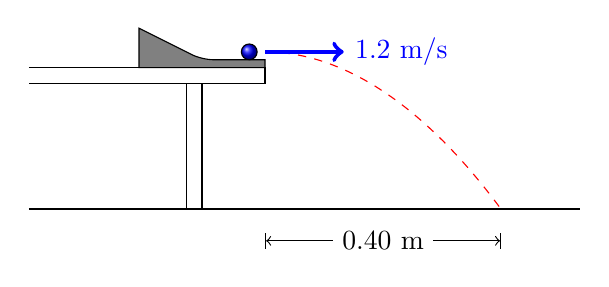
\begin{tikzpicture}
        \draw[thick] (0,0) -- (7,0);
        \draw (0,1.8)
          -- ++ (3,0)
          -- ++ (0,-.2)
          -- ++ (-3,0);
        \draw (2,0) rectangle (2.2,1.6);
        \draw[fill=gray] (3,1.9)
          -- ++(0,-.1)
          -- ++(-1.6,0) 
          -- ++(0,0.5)
          to[rounded corners] ++(.8,-.4)
          -- cycle;
        \draw[shading=ball] (2.8,2) circle (0.1);
        \draw[dashed,red] (3,2) parabola (6,0);
        \draw[blue,ultra thick,->] (3,2) -- ++(1,0) 
          node[anchor=west] {1.2 m/s};
        \draw[|<->|] (3,-.4) -- ++(3,0) 
          node[midway,fill=white] {0.40 m};
  
      \end{tikzpicture}
      \vspace{1em}

    \part
      How much time would the marble be in the air?
      \vs
  
    \part
      From what height should the marble be launched?
      \vs
  
    \part
      What is the $x$- and $y$- velocity of the marble just before hitting the ground?
      \vs
  
    \part
      What is the magnitude and direction of the resultant velocity just before hitting the ground?
      \vs

  \end{parts}

\end{questions}






\end{document}